\documentclass{article}
\usepackage[T1]{fontenc}
\usepackage{lmodern}
\usepackage{graphicx}
\usepackage{amsmath,amssymb}
\usepackage[a4paper,margin=2cm]{geometry}
\usepackage[absolute,overlay]{textpos}
\setlength{\TPHorizModule}{1mm}
\setlength{\TPVertModule}{1mm}
\usepackage[indonesian]{babel}
\usepackage{hyperref}
\setlength{\emergencystretch}{2em}
% unit: Halaman 72

\begin{document}

% === Halaman 72 (python/native) ===

72

\% Ambil hanya bit-bit pesan

vektorBiner = vektorBiner(31:m);


\% Ubah vektor biner ke desimal

for i = 1 : L

    bin(i,:) = vektorBiner((i-1)*8 + 1 : i*8);

dec(i) = bin2dec(num2str(bin(i,:)));

end

pesan = char(dec);


\%Tampilkan pesan

disp('Pesan yang diekstraksi:');

disp(pesan)

>> LSB\_ekstrak

Ketikkan nama file citra stegano: output.bmp

Ekstraksi pesan....

Pesan yang diekstraksi:

Mari kita jaga negara kesatuan Republik Indonesia tercinta. Oke?

Running program:

% deskripsi: gambar native xref 314
\noindent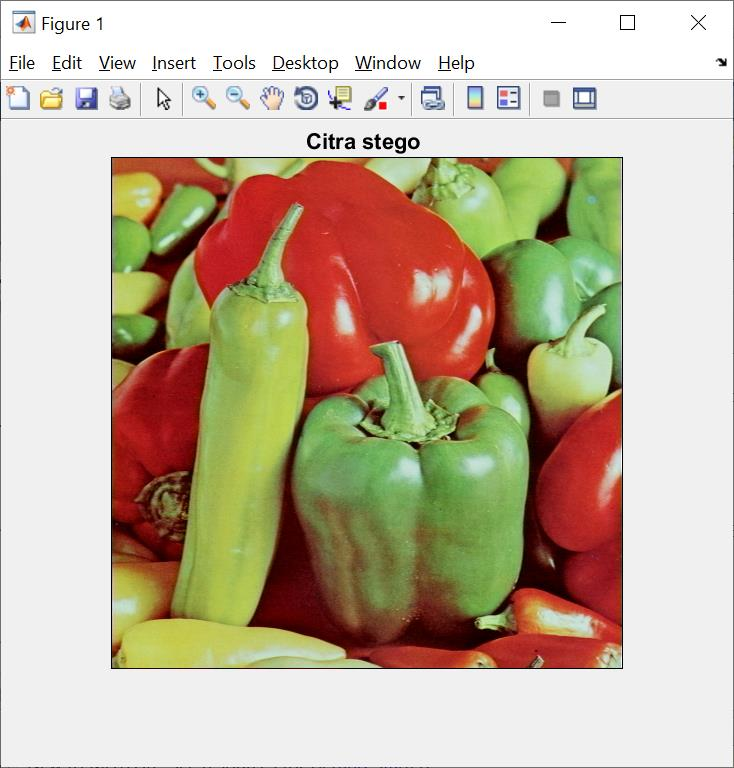
\includegraphics[width=0.85\textwidth]{../../images/python/page_072_img_01.jpeg}

\end{document}
